\documentclass[
	a4paper,
	oneside,
	BCOR = 10mm,
	DIV = 12,
	12pt,
	headings = normal,
]{scrartcl}

%%% Length calculations
\usepackage{calc}
%%%

%%% Support for color
\usepackage{xcolor}
\definecolor{lightblue}{HTML}{03A9F4}
\definecolor{red}{HTML}{F44336}
%%%

%%% Including graphics
\usepackage{graphicx}
%%%

%%% Font selection
\usepackage{fontspec}

\setromanfont{STIX Two Text}[
	SmallCapsFeatures = {LetterSpace = 8},
]

\setsansfont{IBM Plex Sans}[
	Scale = MatchUppercase,
]

\setmonofont{IBM Plex Mono}[
	Scale = MatchUppercase,
]
%%%

%%% Math typesetting
\usepackage{amsmath}

\usepackage{unicode-math}
\setmathfont{STIX Two Math}
%%%

%%% List settings
\usepackage{enumitem}
\setlist[enumerate]{
	label*      = {\arabic*.},
	leftmargin  = *,
	labelindent = \parindent,
	topsep      = 1\baselineskip,
	parsep      = 0\baselineskip,
	itemsep     = 1\baselineskip,
}

\setlist[itemize]{
	label*      = {—},
	leftmargin  = *,
	labelindent = \parindent,
	topsep      = 1\baselineskip,
	parsep      = 0\baselineskip,
	itemsep     = 1\baselineskip,
}

\setlist[description]{
	font        = {\rmfamily\upshape\bfseries},
	topsep      = 1\baselineskip,
	parsep      = 0\baselineskip,
	itemsep     = 0\baselineskip,
}

%%%

%%% Structural elements typesetting
\setkomafont{pagenumber}{\rmfamily}
\setkomafont{disposition}{\rmfamily\bfseries}

% Sectioning
\RedeclareSectionCommand[
	beforeskip = -1\baselineskip,
	afterskip  = 1\baselineskip,
	font       = {\normalsize\bfseries\scshape},
]{section}

\RedeclareSectionCommand[
	beforeskip = -1\baselineskip,
	afterskip  = 1\baselineskip,
	font       = {\normalsize\bfseries\itshape},
]{subsection}

\RedeclareSectionCommand[
	beforeskip = -1\baselineskip,
	afterskip  = 1\baselineskip,
	font       = {\normalsize\bfseries},
]{subsubsection}

\RedeclareSectionCommand[
	beforeskip = -1\baselineskip,
	afterskip  = -0.5em,
	font       = {\normalsize\mdseries\scshape\addfontfeatures{Letters = {UppercaseSmallCaps}}},
]{paragraph}
%%%

%%% Typographic enhancements
\usepackage{microtype}
%%%

%%% Language-specific settings
\usepackage{polyglossia}
\setmainlanguage{ukrainian}
\setotherlanguages{english}
%%%

%%% Captions
\usepackage{caption}
\usepackage{subcaption}

%\DeclareCaptionLabelFormat{closing}{#2)}
%\captionsetup[subtable]{labelformat = closing}

%\captionsetup[subfigure]{labelformat = closing}

\captionsetup[table]{
	aboveskip = 0\baselineskip,
	belowskip = 0\baselineskip,
}

\captionsetup[figure]{
	aboveskip = 1\baselineskip,
	belowskip = 0\baselineskip,
}

\captionsetup[subfigure]{
	labelformat = simple,
	labelformat = brace,
}
%%%

%%% Hyphenated ragged typesetting
\usepackage{ragged2e}
%%%

%%% Table typesetting
\usepackage{booktabs}
\usepackage{longtable}

\usepackage{multirow}

\usepackage{array}
\newcolumntype{v}[1]{>{\RaggedRight\arraybackslash\hspace{0pt}}p{#1}}
\newcolumntype{b}[1]{>{\Centering\arraybackslash\hspace{0pt}}p{#1}}
\newcolumntype{n}[1]{>{\RaggedLeft\arraybackslash\hspace{0pt}}p{#1}}
%%%

%%% Drawing
\usepackage{tikz}
\usepackage{tikzscale}
\usetikzlibrary{positioning}
\usetikzlibrary{arrows.meta} % Stealth arrow tips
%%%

%%% SI units typesetting
\usepackage{siunitx}
\sisetup{
	output-decimal-marker = {,},
	exponent-product      = {\cdot},
	inter-unit-product    = \ensuremath{{} \cdot {}},
	per-mode              = symbol,
}
%%%

%%% Links and hyperreferences
\usepackage{hyperref}
\hypersetup{
	bookmarksnumbered = true,
	colorlinks      = false,
	linkbordercolor = red,
	urlbordercolor  = lightblue,
	pdfborderstyle  = {/S/U/W 1.5},
}
%%%

%%% Length adjustments
% Set baselineskip, default is 14.5 pt
\linespread{1.068966} % ~15.5 pt
\setlength{\emergencystretch}{1em}
\setlength{\parindent}{1.5em}
\newlength{\gridunitwidth}
\setlength{\gridunitwidth}{\textwidth / 12}
%%%

%%% Custom commands
\newcommand{\allcaps}[1]{{\addfontfeatures{LetterSpace = 8, Kerning = Off}#1}}
%%%

\begin{document}

\begin{titlepage}
		\begin{center}
			Міністерство освіти і науки України\\
			Національний авіаційний університет\\
			Навчально-науковий інститут комп'ютерних інформаційних технологій\\
			Кафедра комп'ютеризованих систем управління

			\vspace{\fill}
				Лабораторна робота №1\\
				з дисципліни «Технології мультимедіа»\\
				на тему «Ознайомлення з~інтерфейсом~\textenglish{Adobe Photoshop}.\\ Корекція колірного і~тонового балансу зображень»\\

			\vspace{\fill}

			\begin{flushright}
				Виконав:\\
				студент \allcaps{ННІКІТ}\\
				групи СП-325\\
				Клокун В.\,Д.\\
				Перевірив:\\
				Кашкевич І.\,Ф.
			\end{flushright}

			Київ 2018
		\end{center}
	\end{titlepage}

	\section{Мета роботи}
		Вивчити інтерфейс програми~\textenglish{Adobe Photoshop}, ознайомитись з~основними інструментами для~редагування зображень.

	\section{Завдання роботи}
		Ознайомитись з~основними групами інструментів \textenglish{Adobe Photoshop}, освоїти інструменти виділення, обрізання і~переміщення об'\-єк\-тів та~корекції колірного і~тонового балансу зображень.

	\section{Хід роботи}
		\paragraph{Коригування кольору зображення за~допомогою команди~\textenglish{«Hue/\-Sat\-u\-ra\-tion»}}
			Створюємо шар з~назвою~\textenglish{«Hue-\-Sat\-u\-ra\-tion»} та~виконуємо над~ним команду~\textenglish{«Hue/\-Sat\-u\-ra\-tion»} з~параметром~\textenglish{«Colorize»}~(рис.~\ref{fig:01-huesat}).
			\begin{figure}[!htbp]
				\centering
				\begin{subfigure}{0.5\columnwidth}
					\centering
					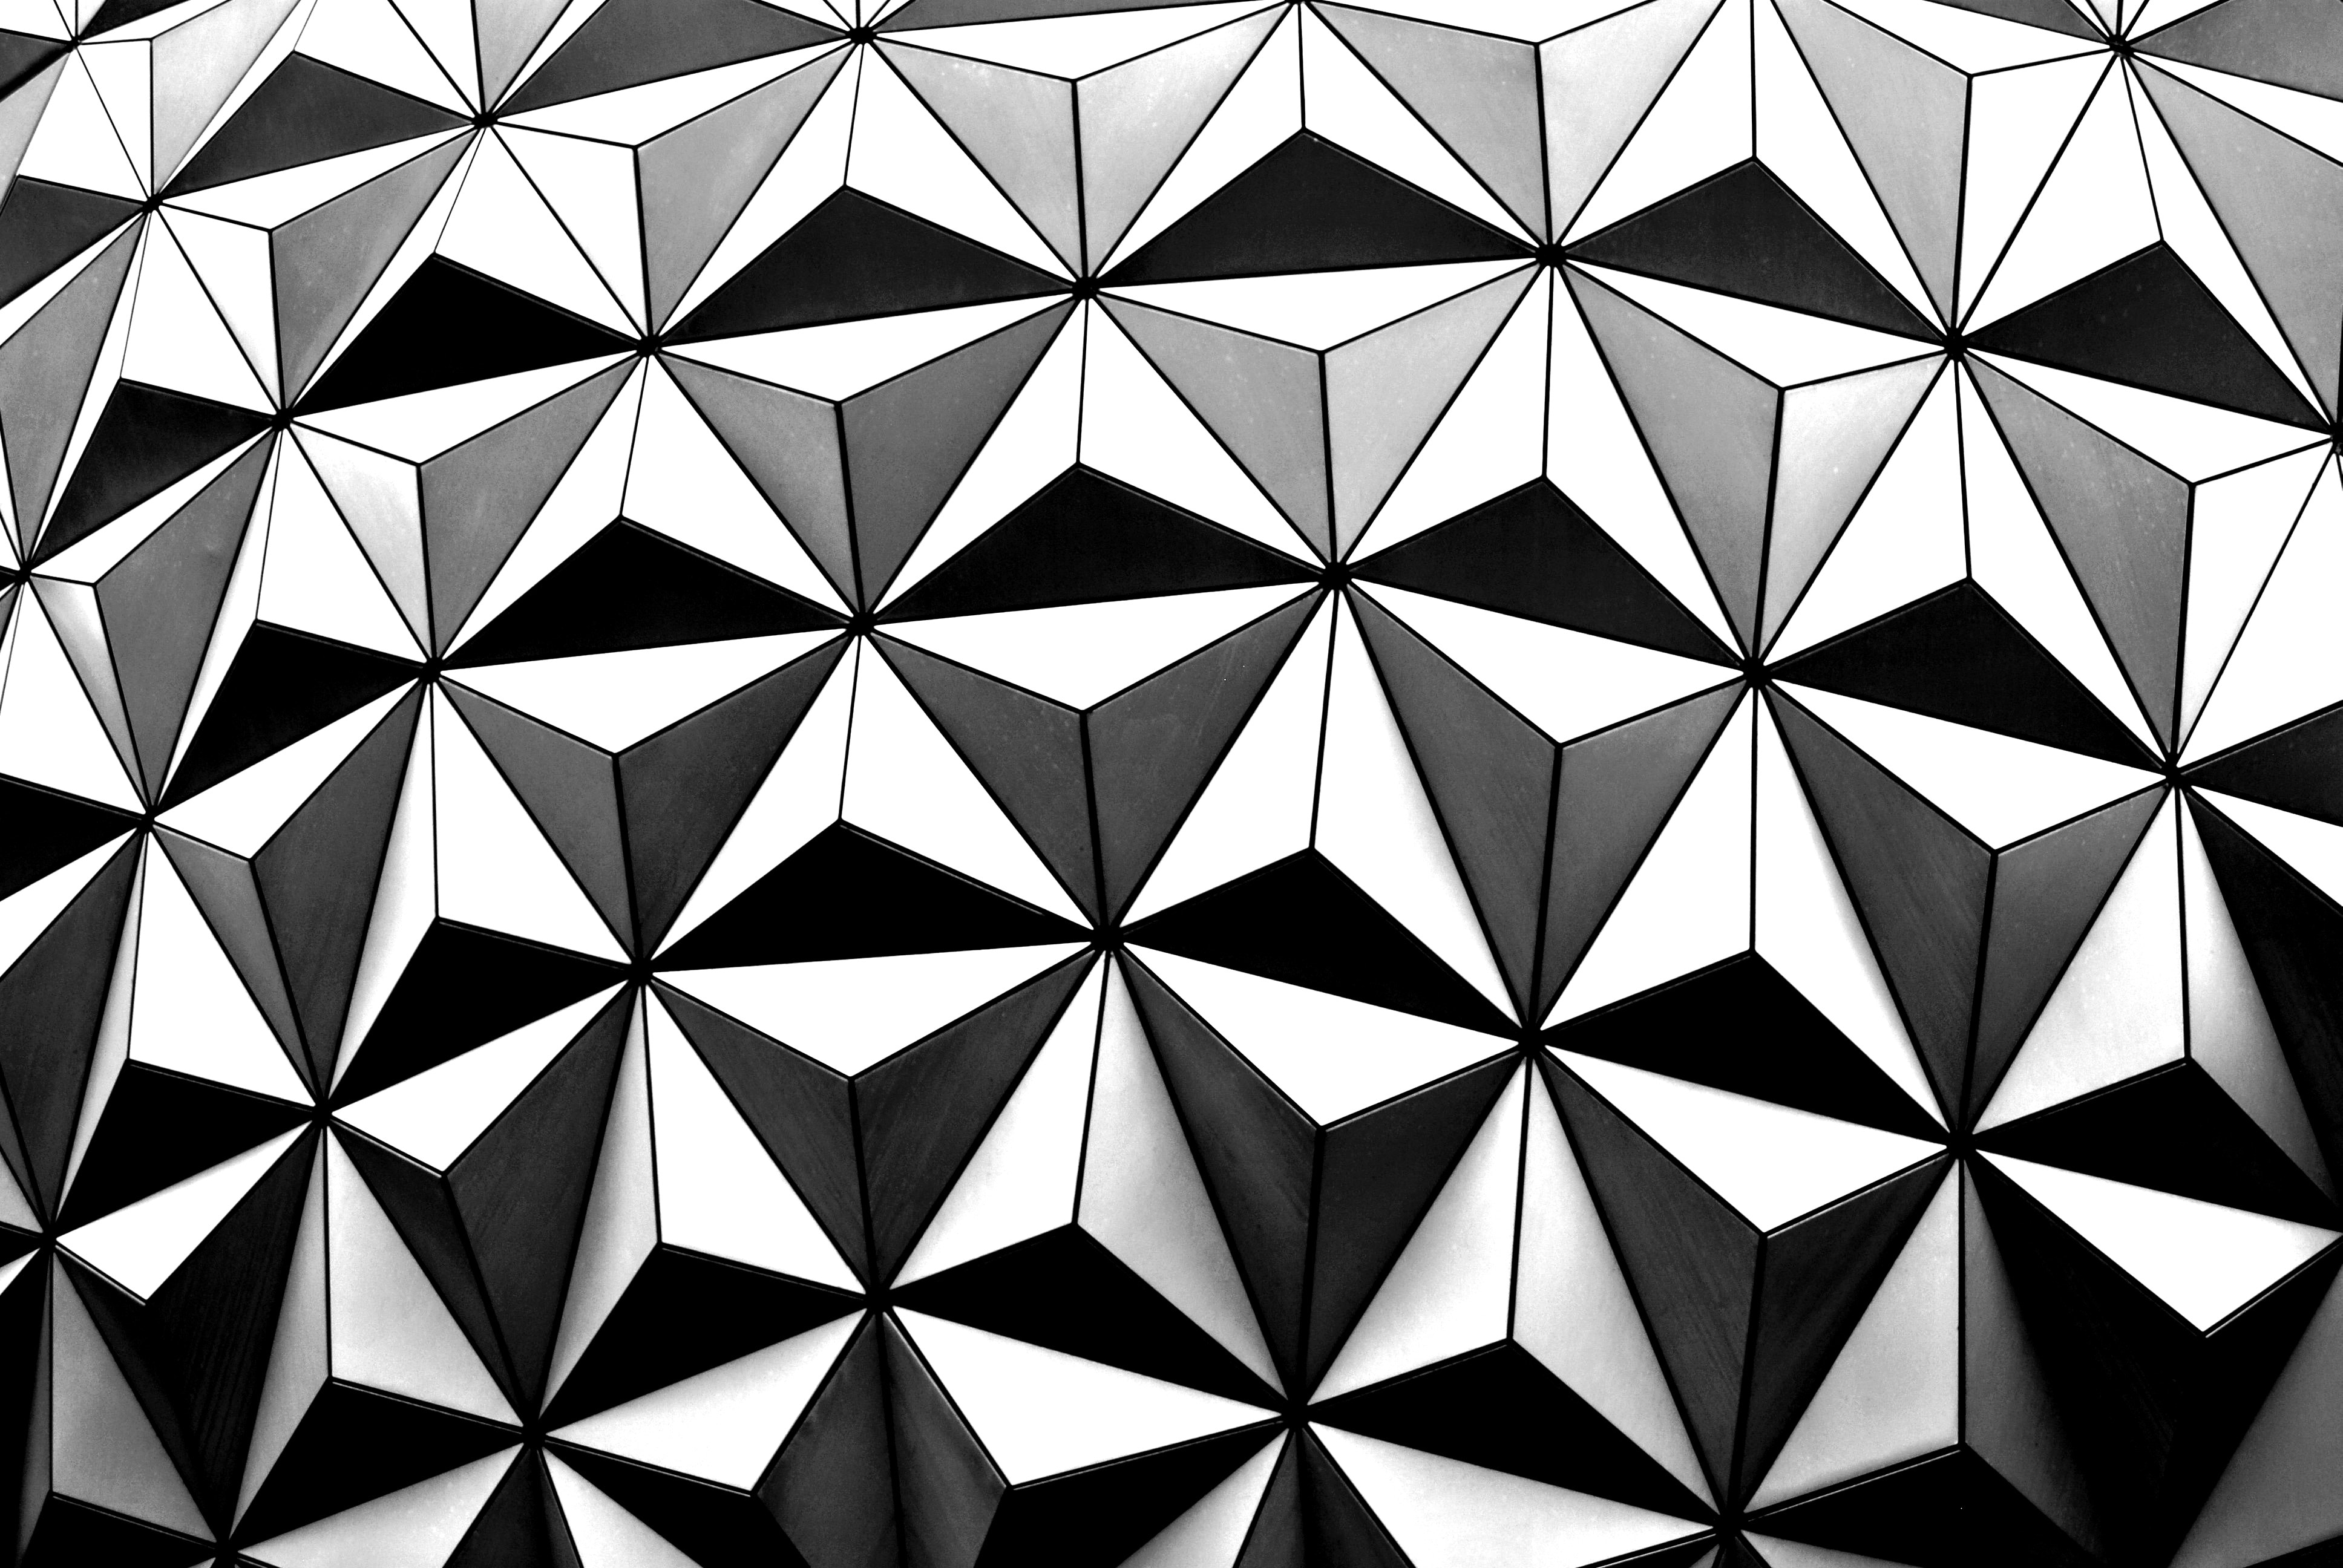
\includegraphics[height = 6\baselineskip]{./assets/abstract-abstract-photo-art-1070345.jpg}
					\caption{}
					\label{subfig:01-01-huesat}
				\end{subfigure}%
				\begin{subfigure}{0.5\columnwidth}
					\centering
					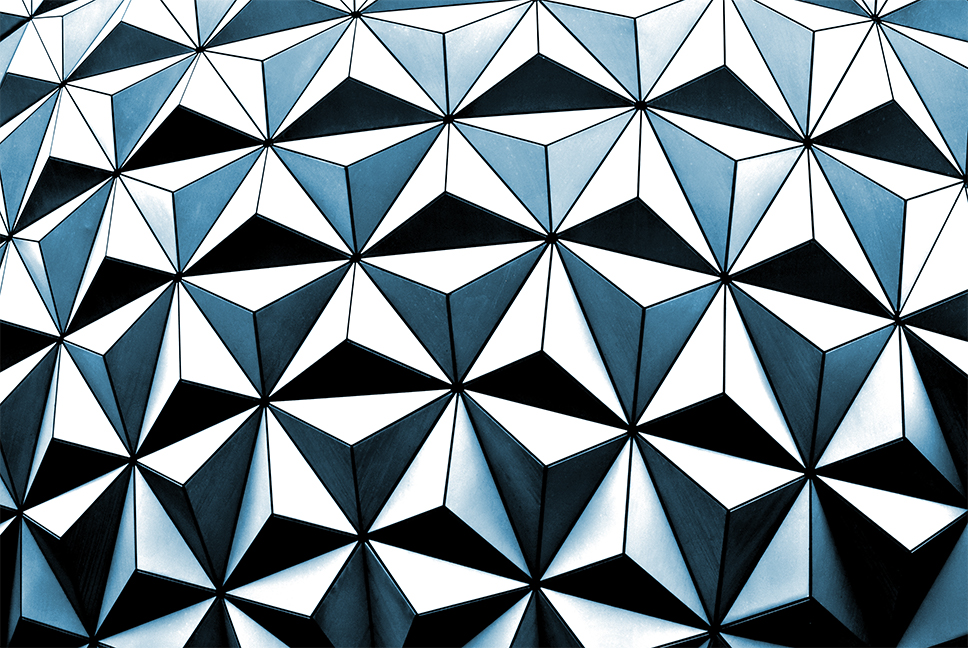
\includegraphics[height = 6\baselineskip]{./assets/y03s01-multimedia-lab-01-p01-01-huesat.jpg}
					\caption{}
					\label{subfig:01-02-huesat}
				\end{subfigure}%
				\caption{Результат роботи команди~\textenglish{«Hue/Saturation»}: \subref{subfig:01-01-huesat}~— до, \subref{subfig:01-02-huesat}~— після}
				\label{fig:01-huesat}
			\end{figure}

		\paragraph{Налаштування відтінків зображення}
			Створюємо шар під~назвою~\textenglish{«Levels»} та~виконуємо над~ним команду~\textenglish{«Levels»}~(рис.~\ref{fig:02-levels}).
			\begin{figure}[!htbp]
				\centering
				\begin{subfigure}{0.5\columnwidth}
					\centering
					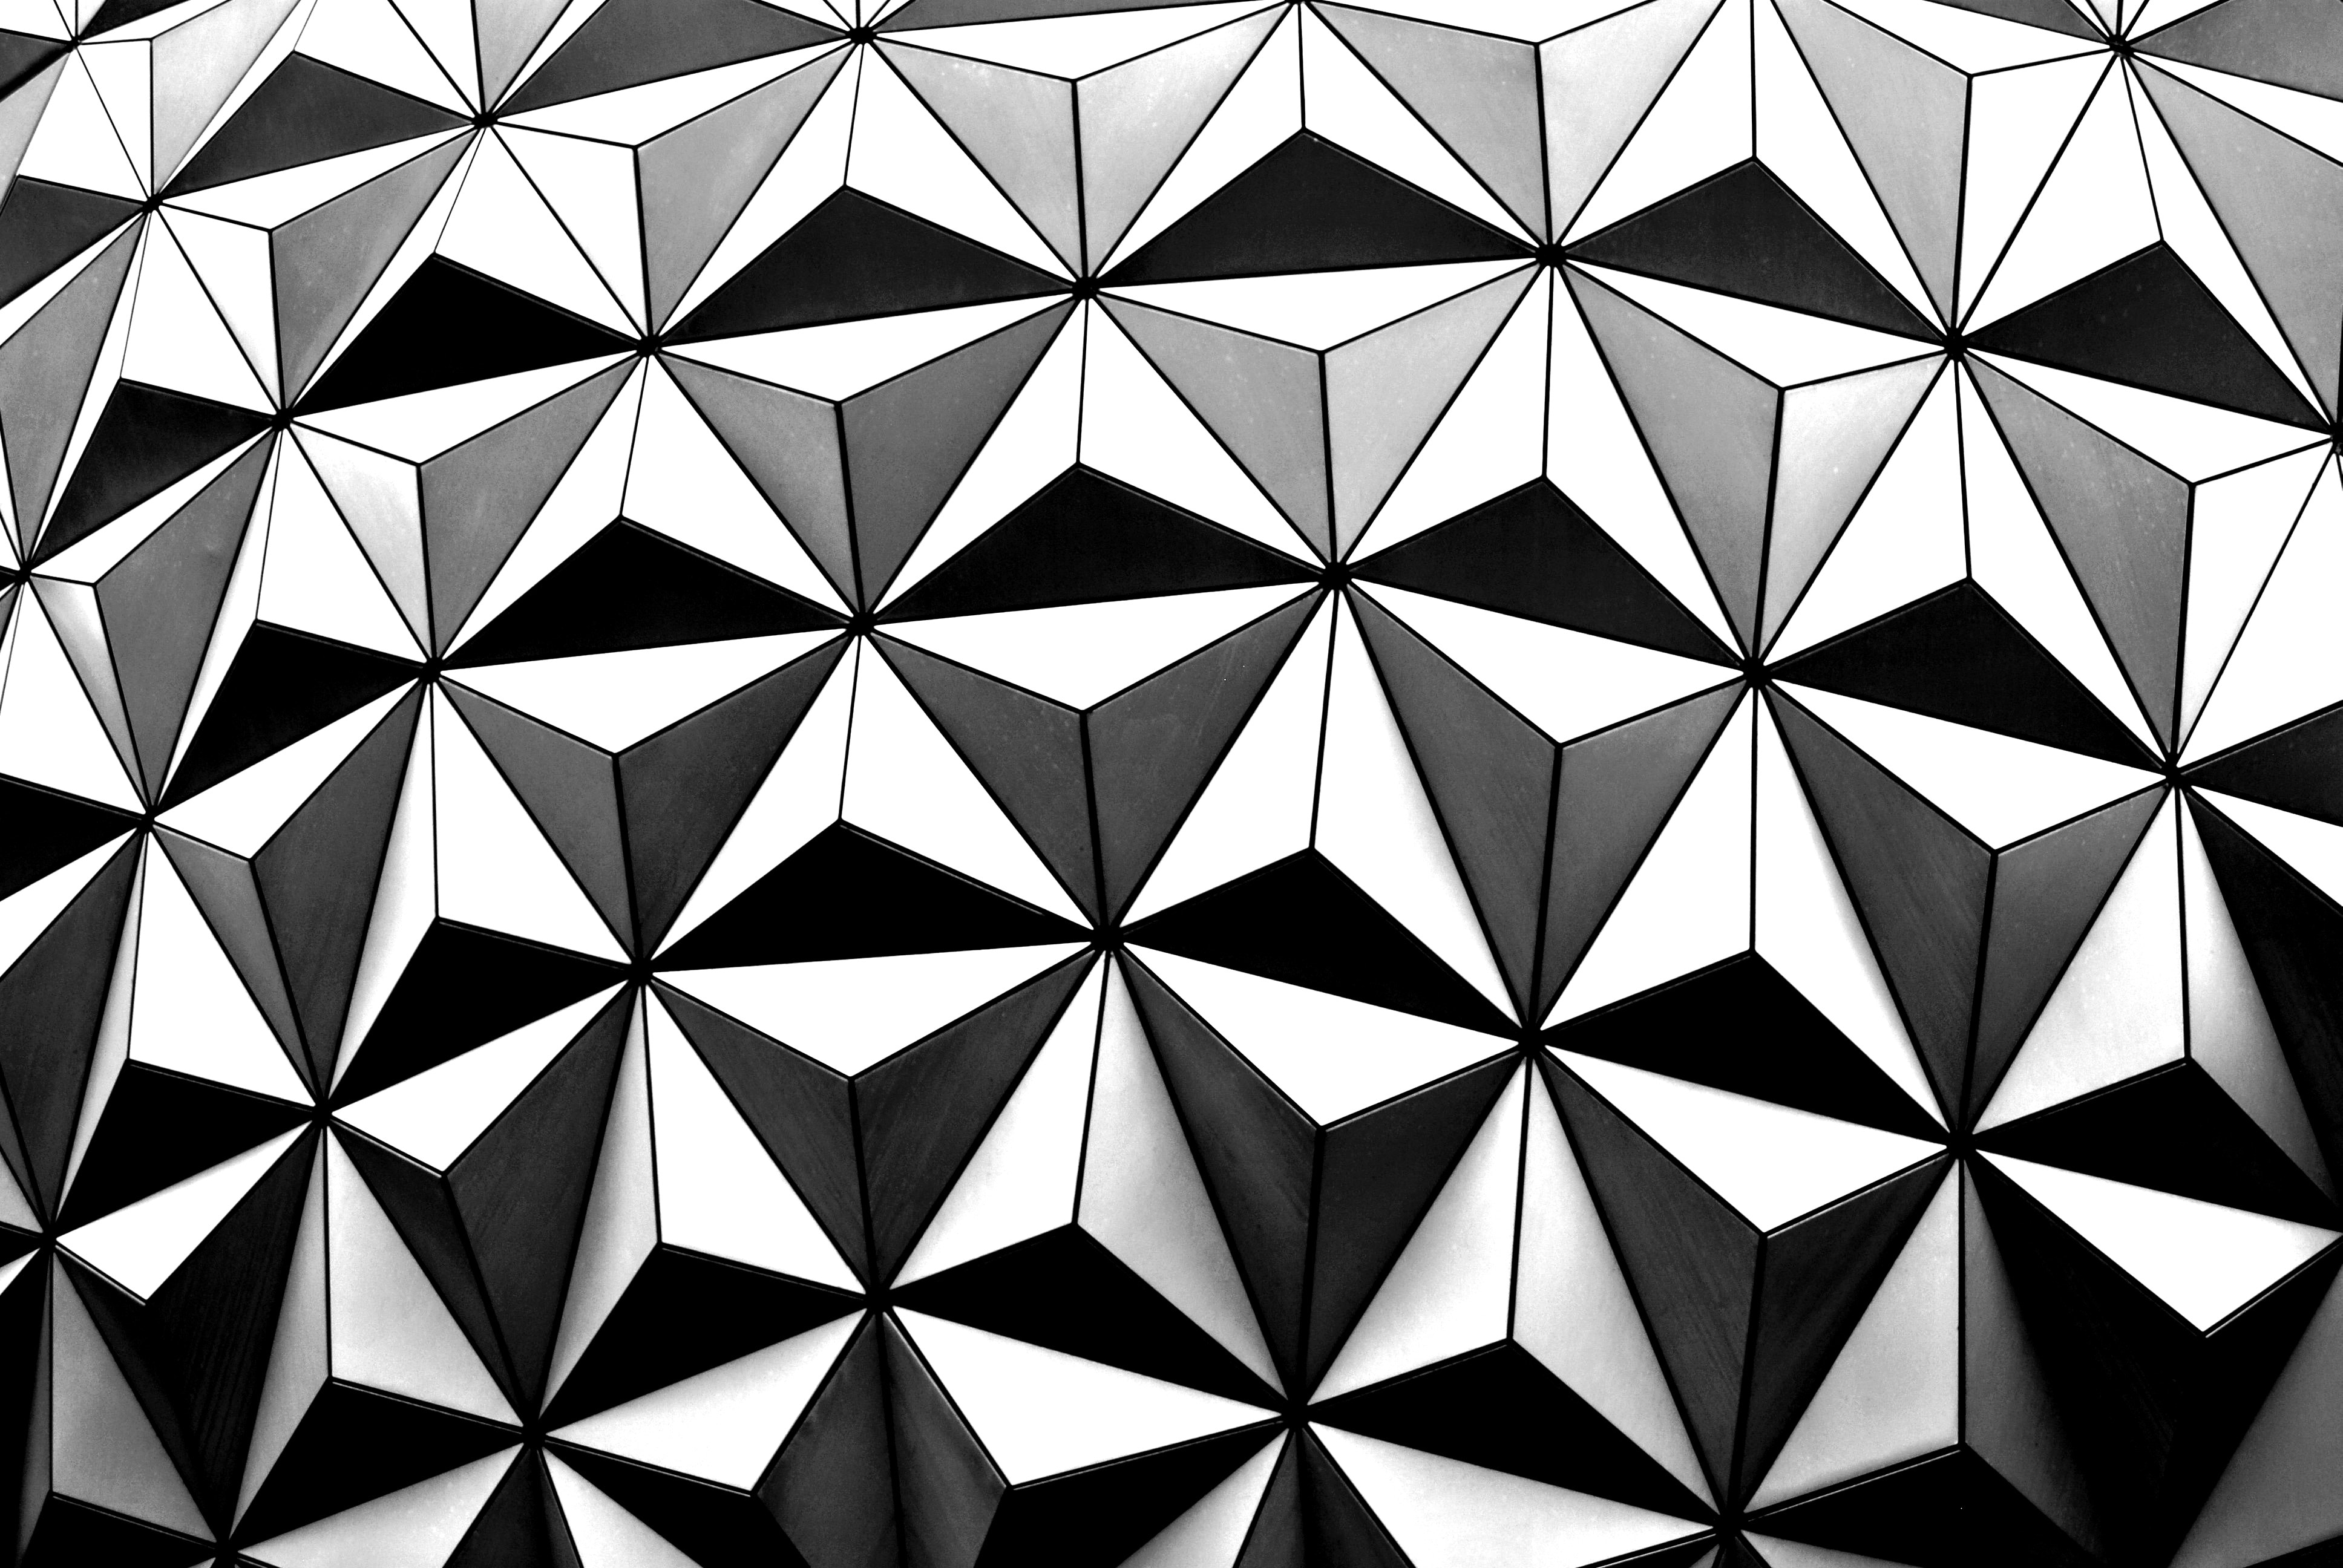
\includegraphics[height = 6\baselineskip]{./assets/abstract-abstract-photo-art-1070345.jpg}
					\caption{}
					\label{subfig:02-01-levels}
				\end{subfigure}%
				\begin{subfigure}{0.5\columnwidth}
					\centering
					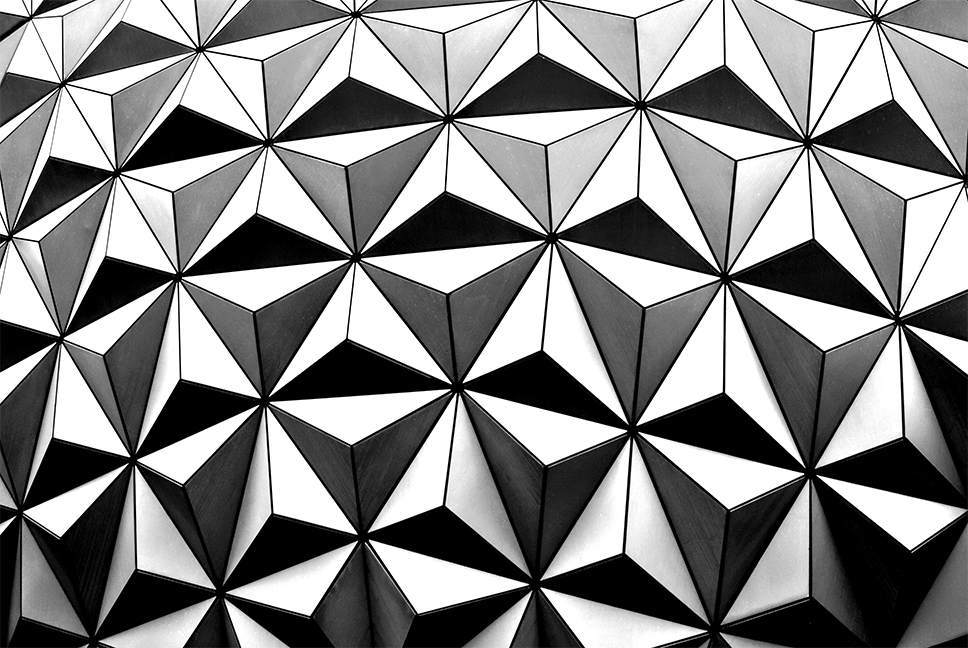
\includegraphics[height = 6\baselineskip]{./assets/y03s01-multimedia-lab-01-p01-02-levels.jpg}
					\caption{}
					\label{subfig:02-02-levels}
				\end{subfigure}%
				\caption{Результат роботи команди~\textenglish{«Levels»}: \subref{subfig:02-01-levels}~— до, \subref{subfig:02-02-levels}~— після}
				\label{fig:02-levels}
			\end{figure}

		\paragraph{Кадрування}
			Виконуємо кадрування зображення за~допомогою інструменту~\textenglish{«Crop»}~(рис.~\ref{fig:03-crop}).
			\begin{figure}[!htbp]
				\centering
				\begin{subfigure}{0.5\columnwidth}
					\centering
					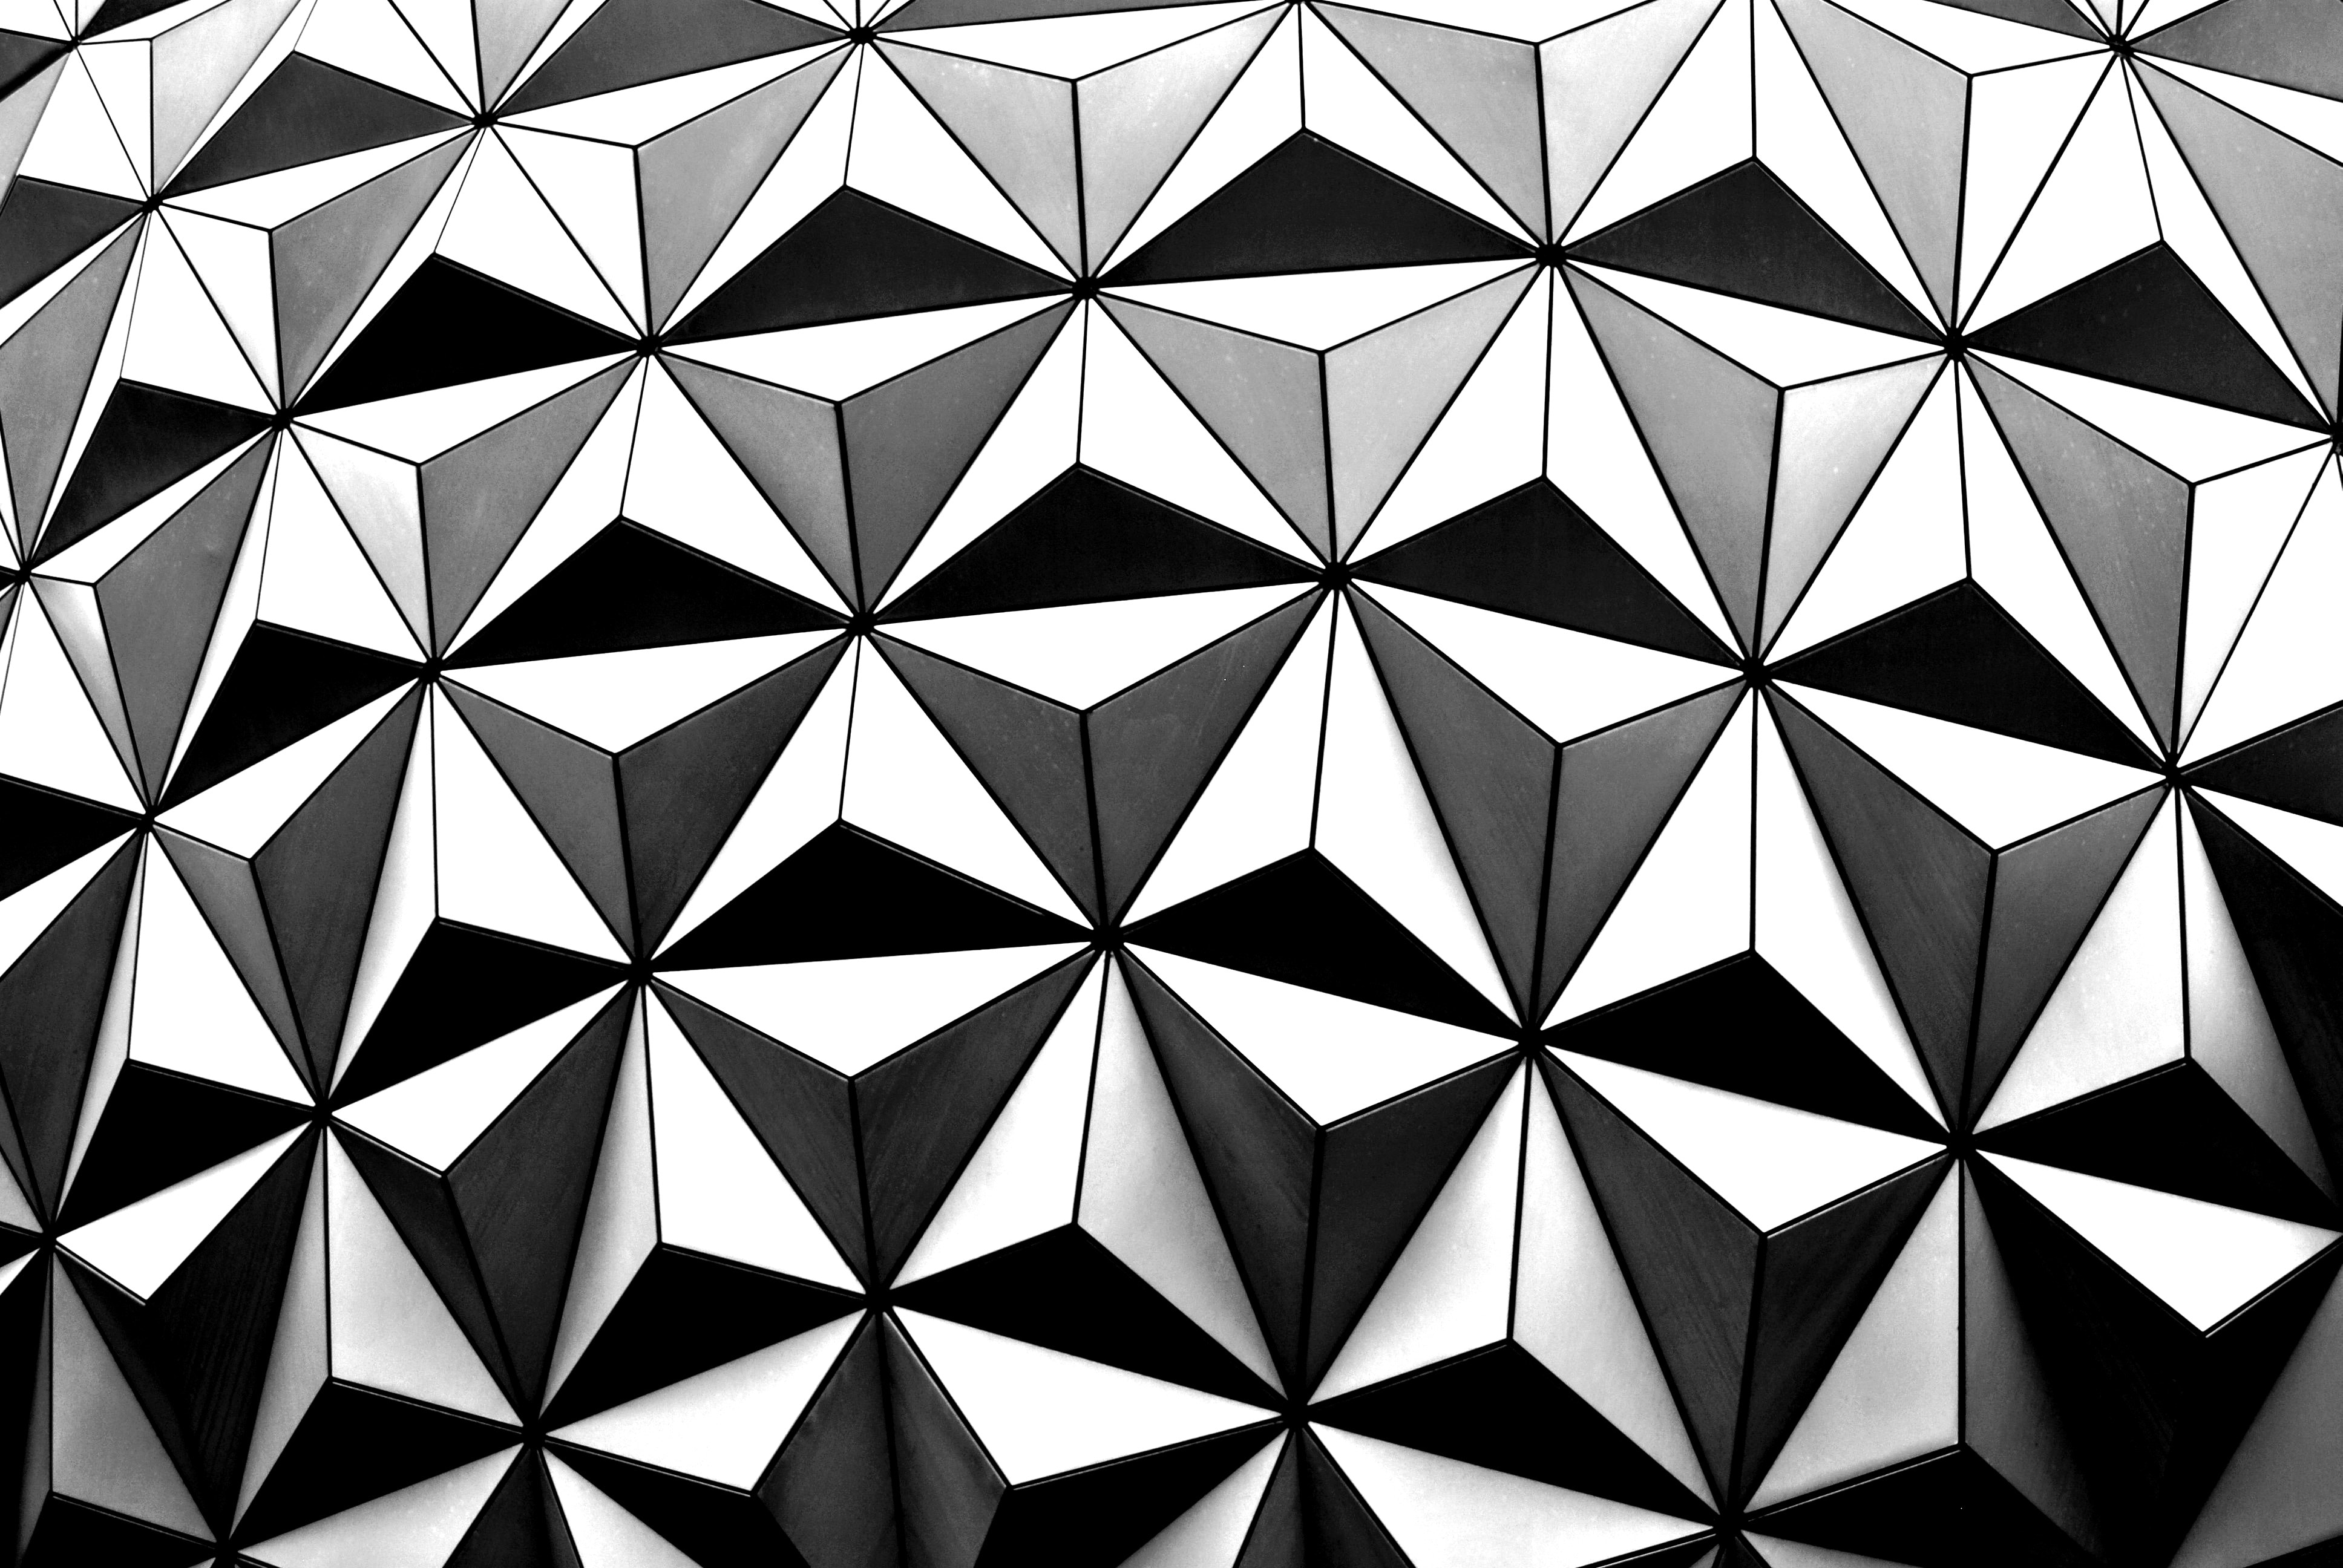
\includegraphics[height = 6\baselineskip]{./assets/abstract-abstract-photo-art-1070345.jpg}
					\caption{}
					\label{subfig:03-01-crop}
				\end{subfigure}%
				\begin{subfigure}{0.5\columnwidth}
					\centering
					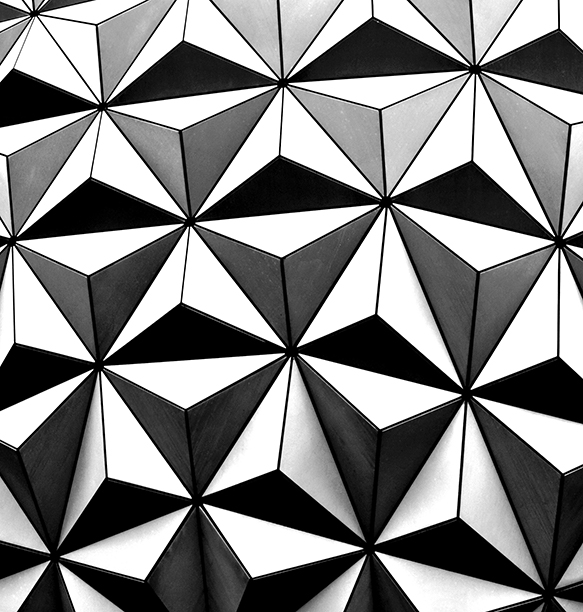
\includegraphics[height = 6\baselineskip]{./assets/y03s01-multimedia-lab-01-p01-03-crop.jpg}
					\caption{}
					\label{subfig:03-02-crop}
				\end{subfigure}%
				\caption{Результат кадрування: \subref{subfig:03-01-crop}~— до, \subref{subfig:03-02-crop}~— після}
				\label{fig:03-crop}
			\end{figure}

		\paragraph{Розмиття}
			Створюємо шар під~назвою~\textenglish{«Blur»} та~виконуємо над~ним операцію~\textenglish{«Blur»}~(рис.~\ref{fig:04-blur}).
			\begin{figure}[!htbp]
				\centering
				\begin{subfigure}{0.5\columnwidth}
					\centering
					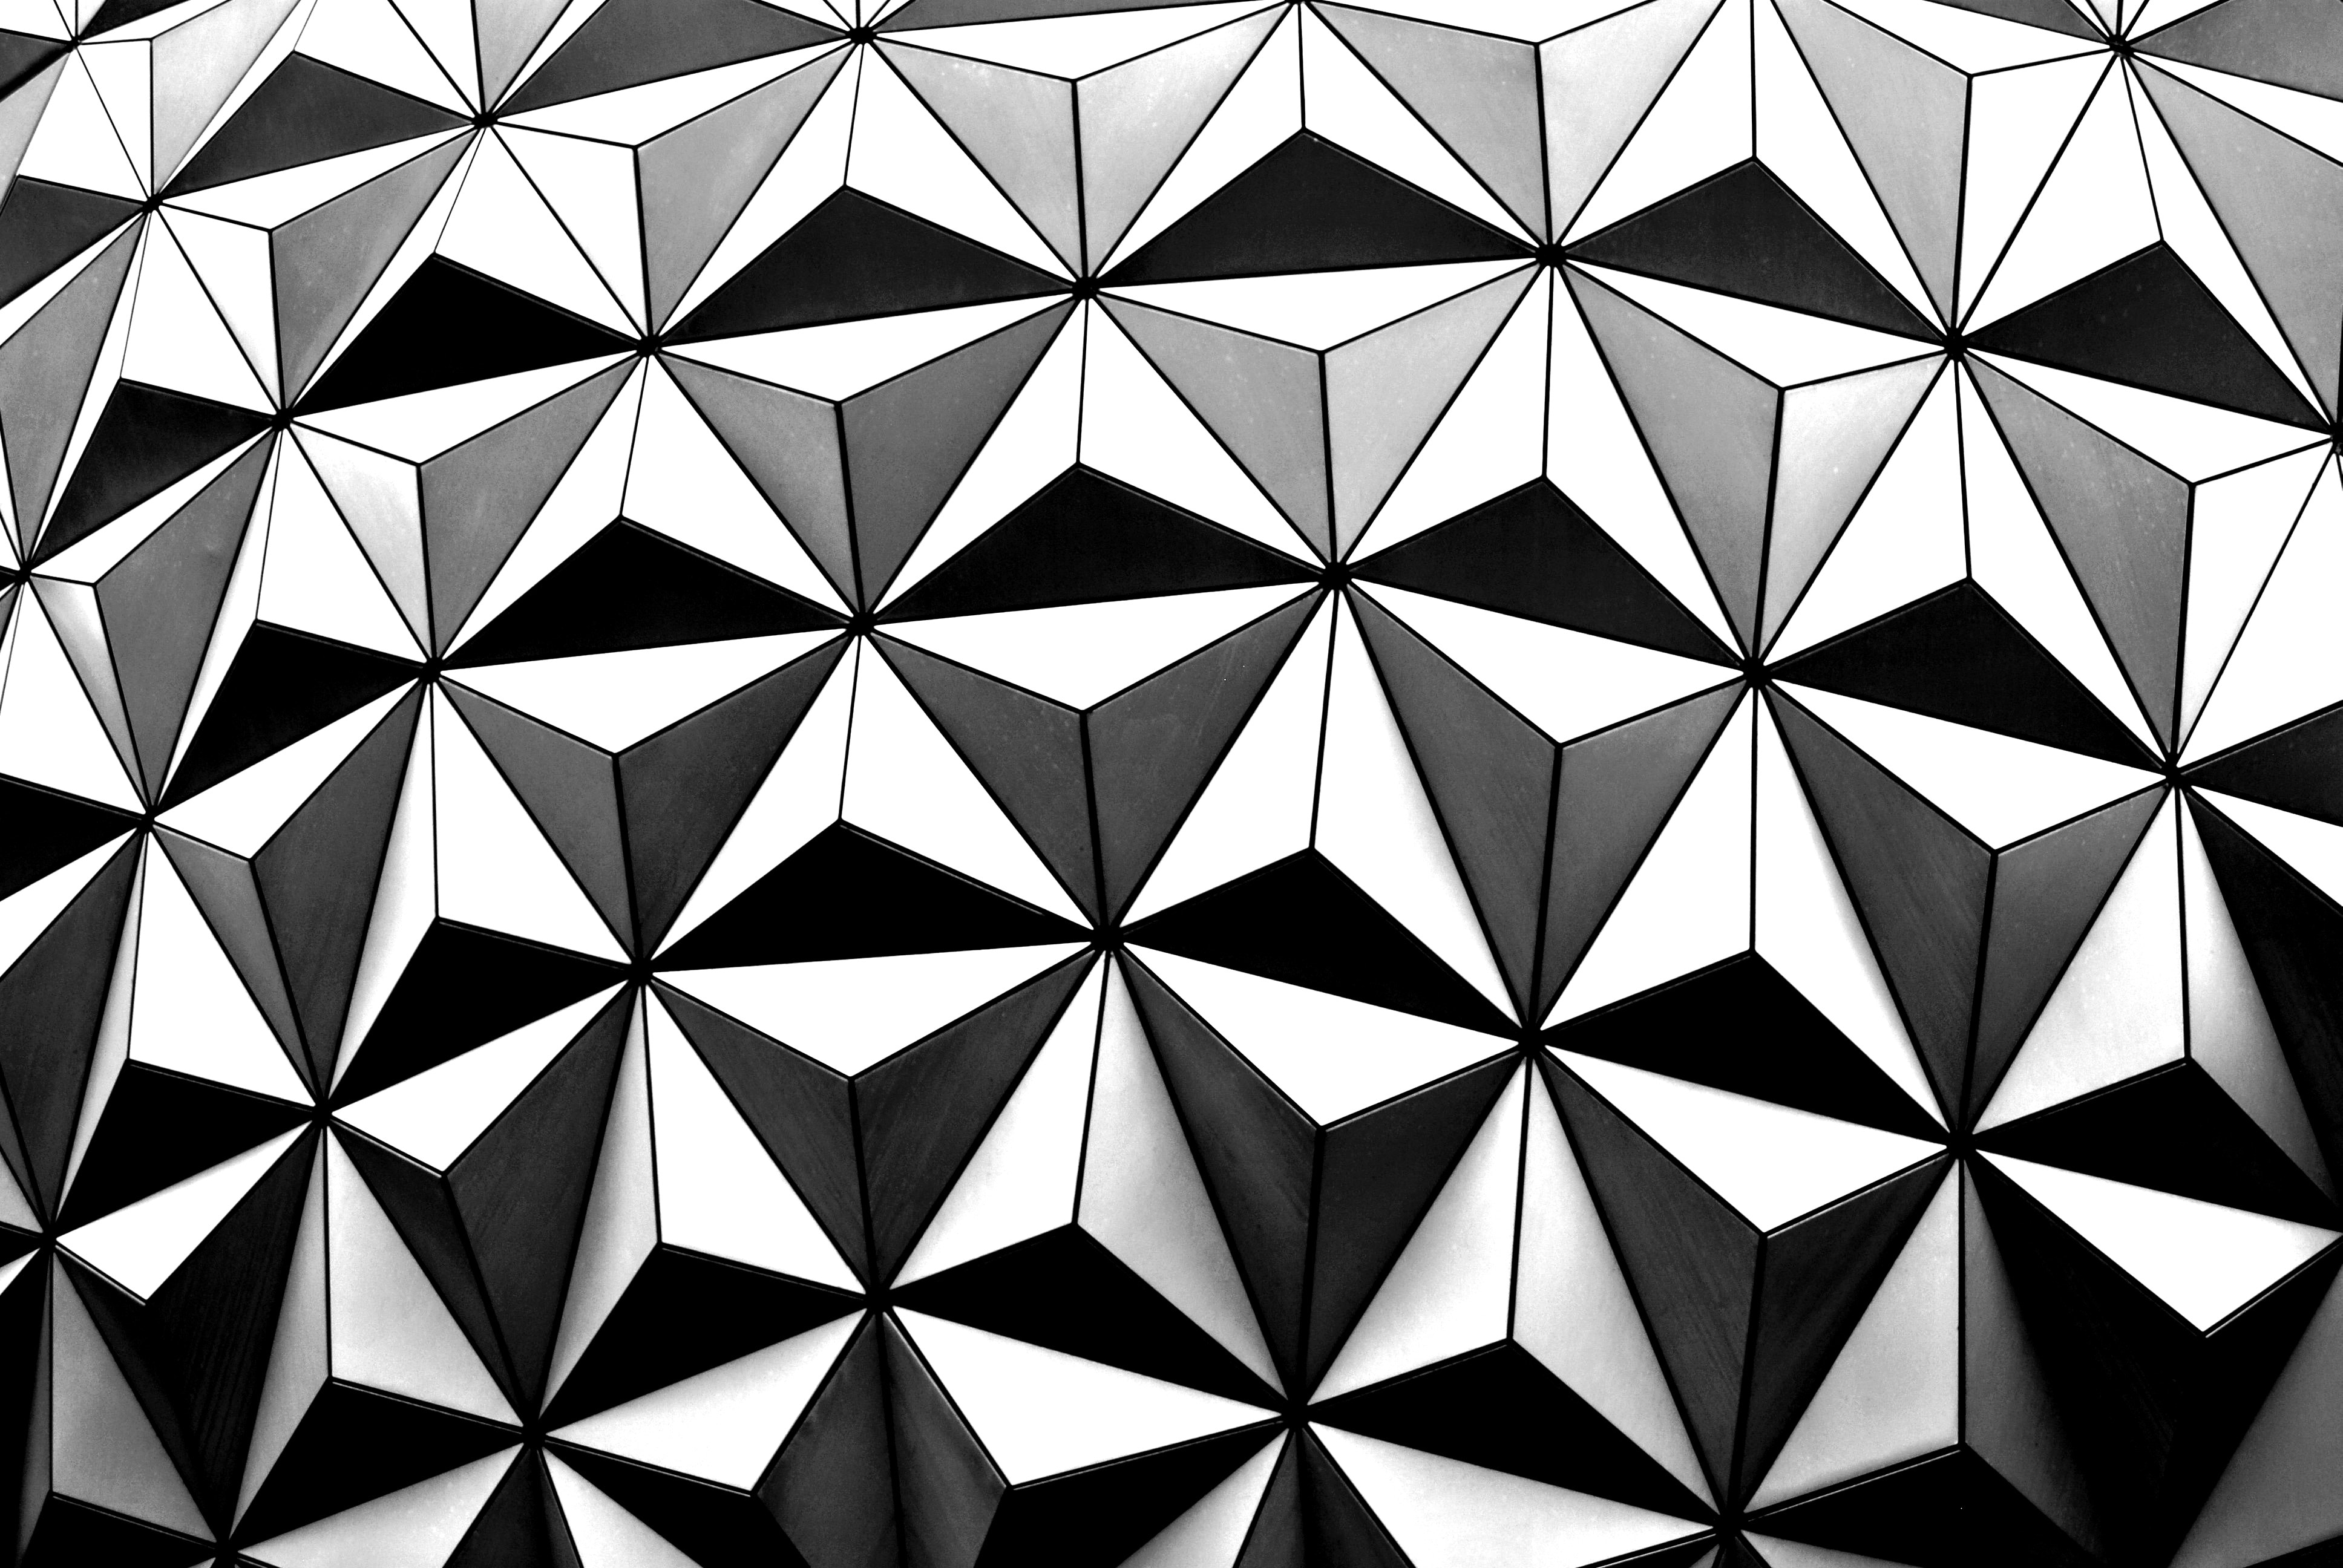
\includegraphics[height = 6\baselineskip]{./assets/abstract-abstract-photo-art-1070345.jpg}
					\caption{}
					\label{subfig:04-01-blur}
				\end{subfigure}%
				\begin{subfigure}{0.5\columnwidth}
					\centering
					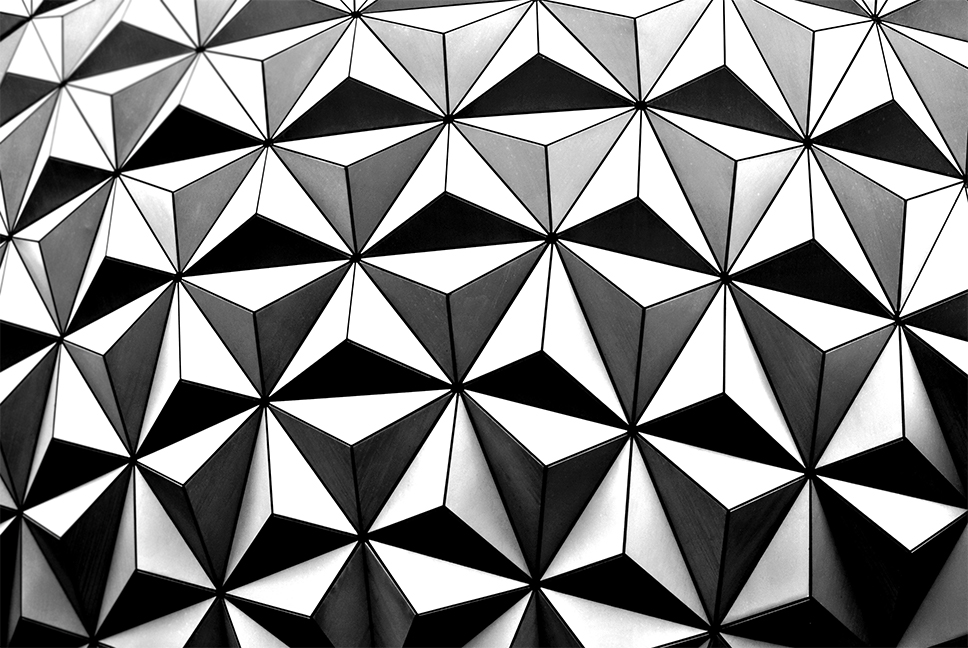
\includegraphics[height = 6\baselineskip]{./assets/y03s01-multimedia-lab-01-p01-04-blur.jpg}
					\caption{}
					\label{subfig:04-02-blur}
				\end{subfigure}%
				\caption{Результат роботи команди~\textenglish{«Blur»}: \subref{subfig:04-01-blur}~— до, \subref{subfig:04-02-blur}~— після}
				\label{fig:04-blur}
			\end{figure}

		\paragraph{Різкість}
			Створюємо шар під~назвою~\textenglish{«Sharpen»} та~виконуємо над~ним операцію~\textenglish{«Sharpen»}~(рис.~\ref{fig:05-sharpen}).
			\begin{figure}[!htbp]
				\centering
				\begin{subfigure}{0.5\columnwidth}
					\centering
					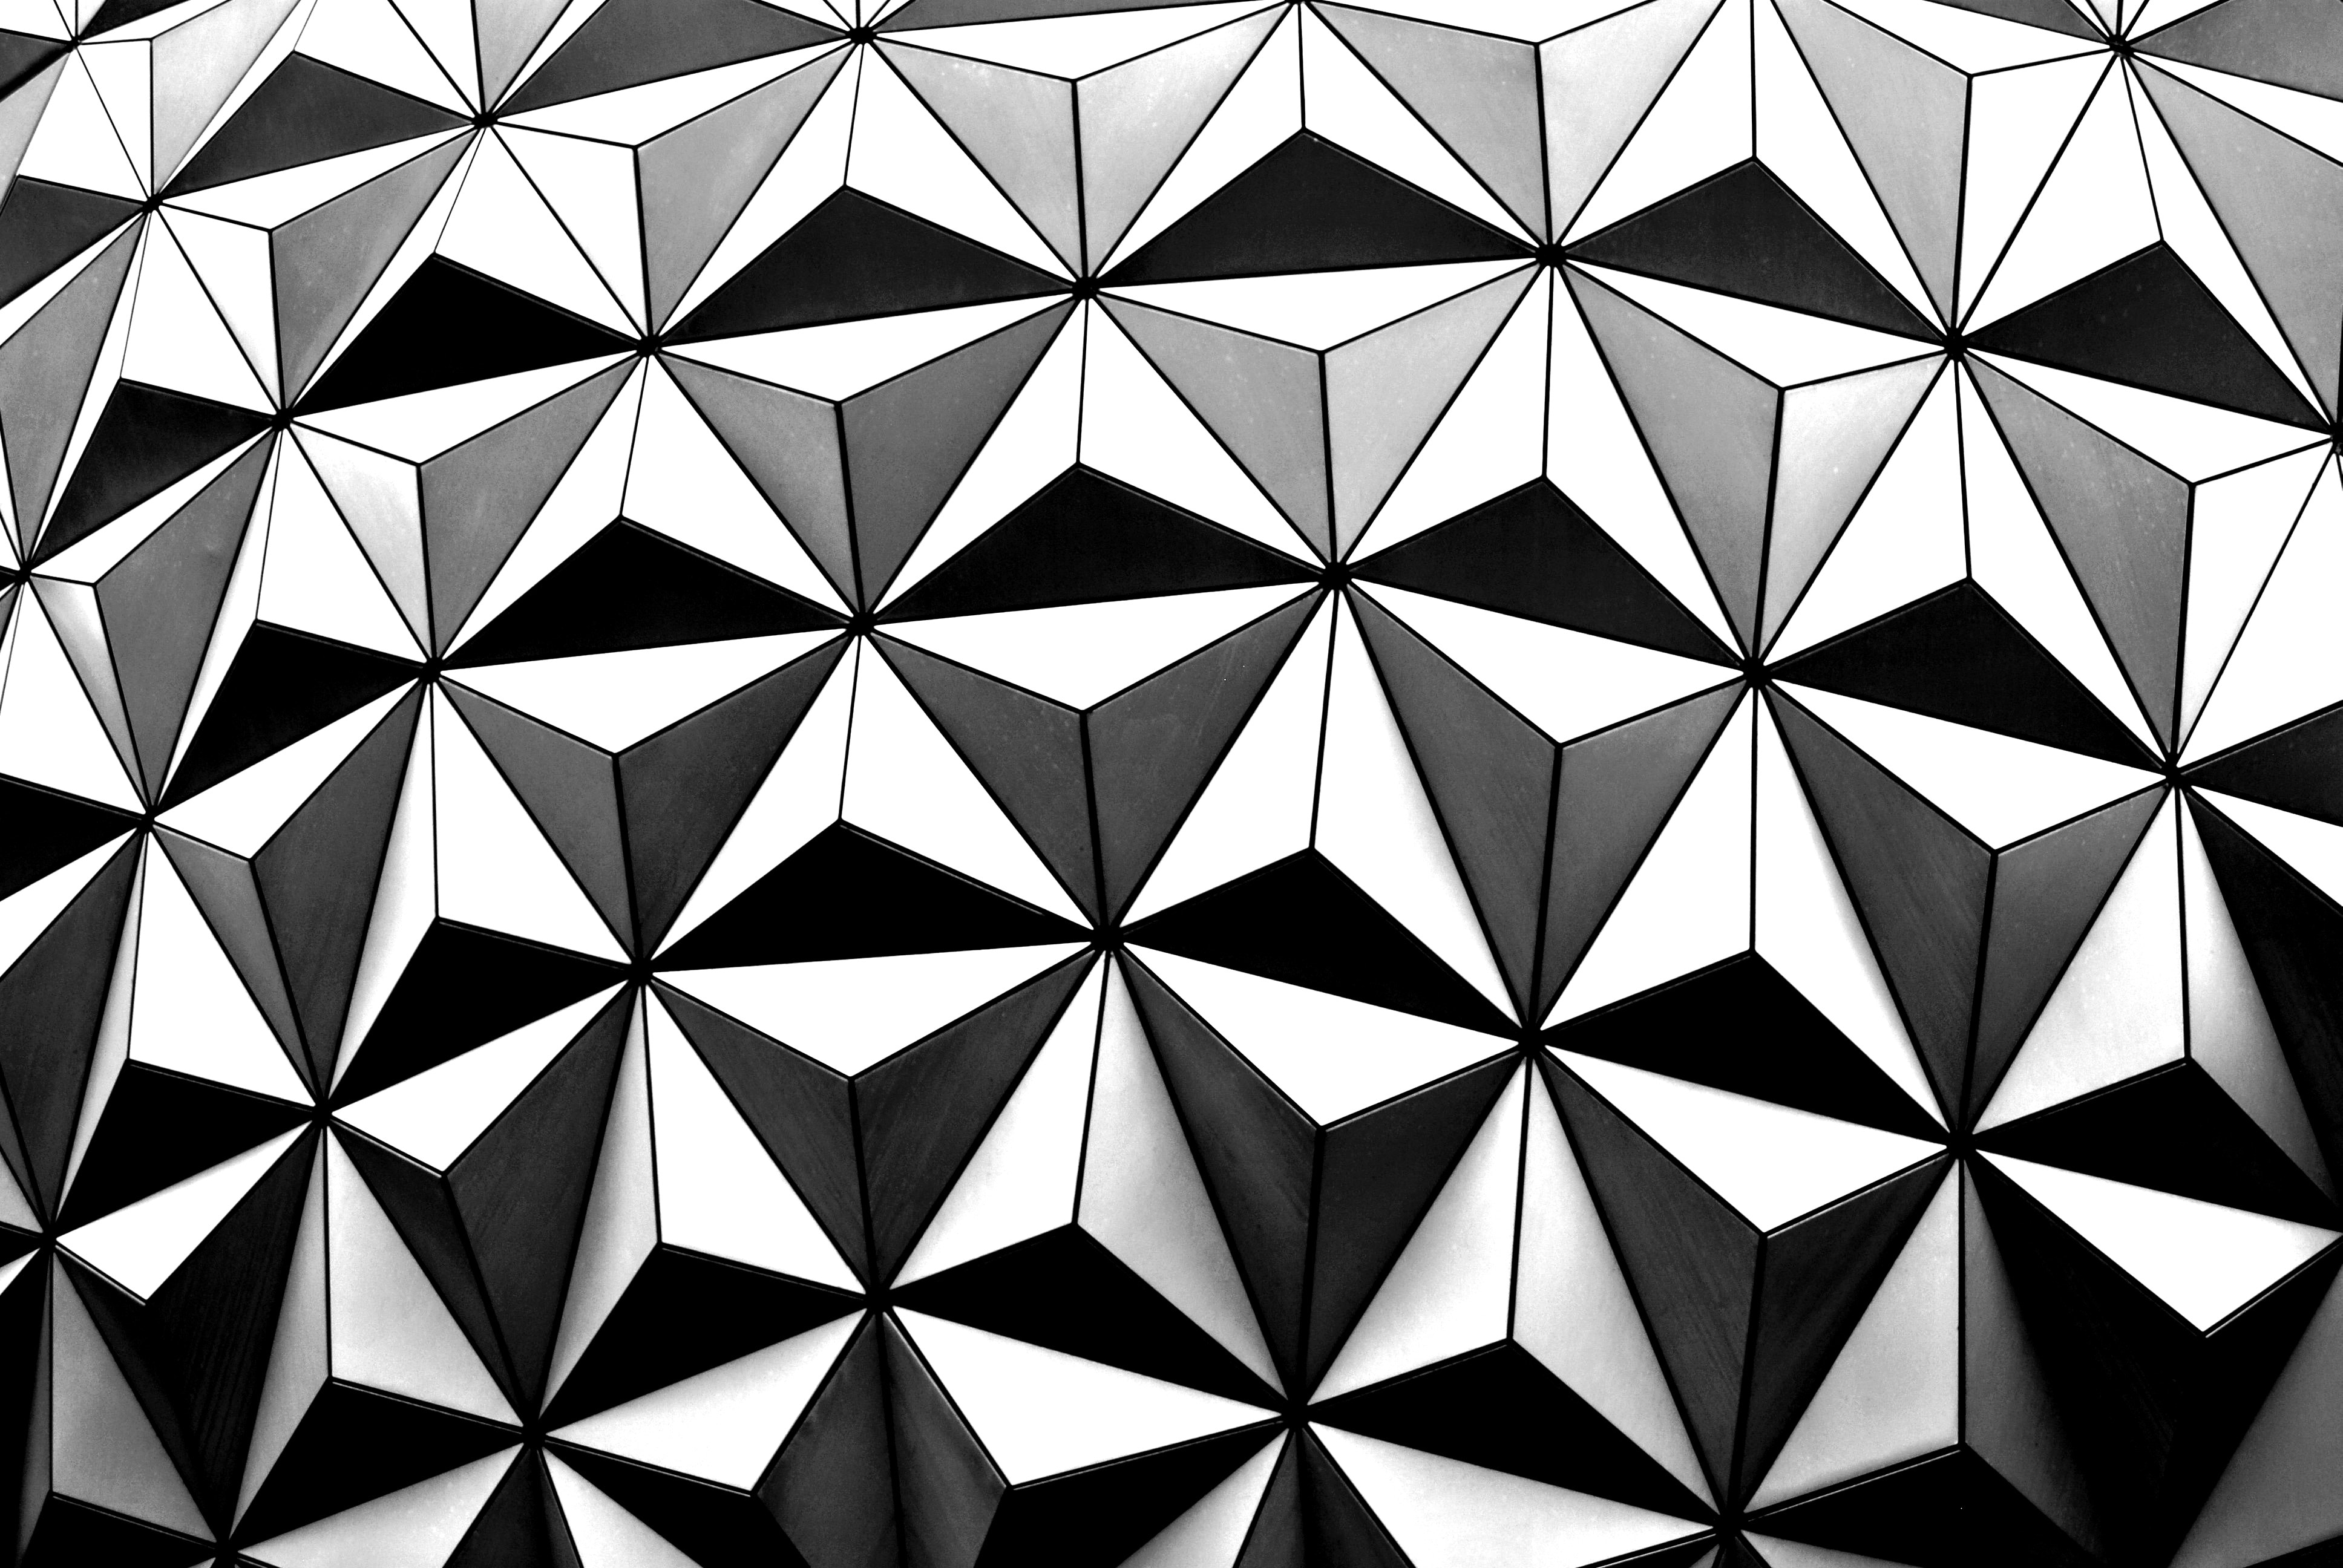
\includegraphics[height = 6\baselineskip]{./assets/abstract-abstract-photo-art-1070345.jpg}
					\caption{}
					\label{subfig:05-01-sharpen}
				\end{subfigure}%
				\begin{subfigure}{0.5\columnwidth}
					\centering
					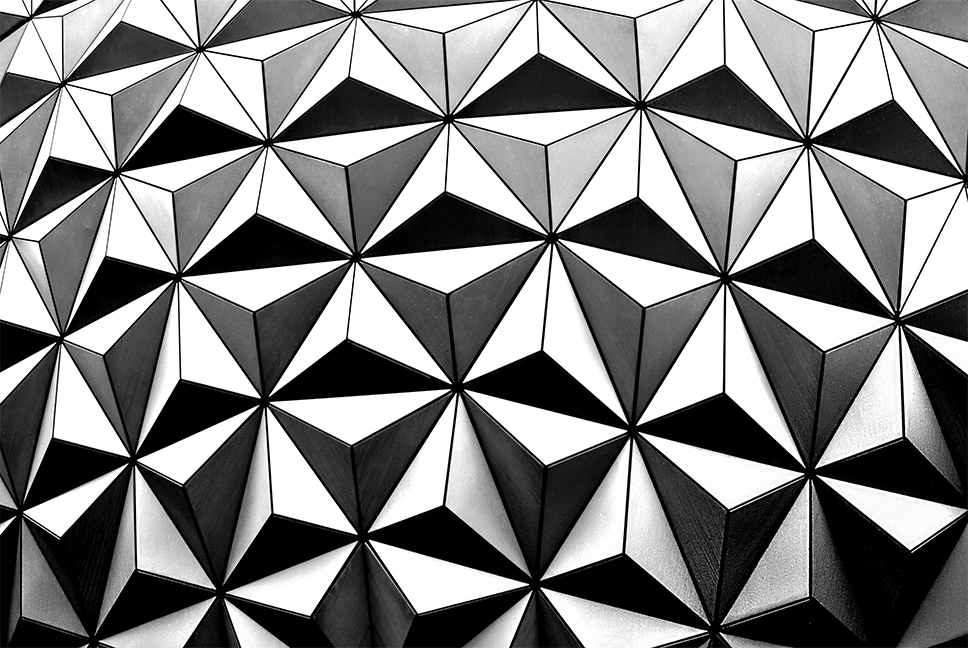
\includegraphics[height = 6\baselineskip]{./assets/y03s01-multimedia-lab-01-p01-05-sharpen.jpg}
					\caption{}
					\label{subfig:05-02-sharpen}
				\end{subfigure}%
				\caption{Результат роботи команди~\textenglish{«Sharpen»}: \subref{subfig:05-01-sharpen}~— до, \subref{subfig:05-02-sharpen}~— після}
				\label{fig:05-sharpen}
			\end{figure}

		\paragraph{Губка}
			Створюємо шар під~назвою~\textenglish{«Sponge»} та~виконуємо над~ним операцію~\textenglish{«Sponge»}~(рис.~\ref{fig:06-sponge}).
			\begin{figure}[!htbp]
				\centering
				\begin{subfigure}{0.5\columnwidth}
					\centering
					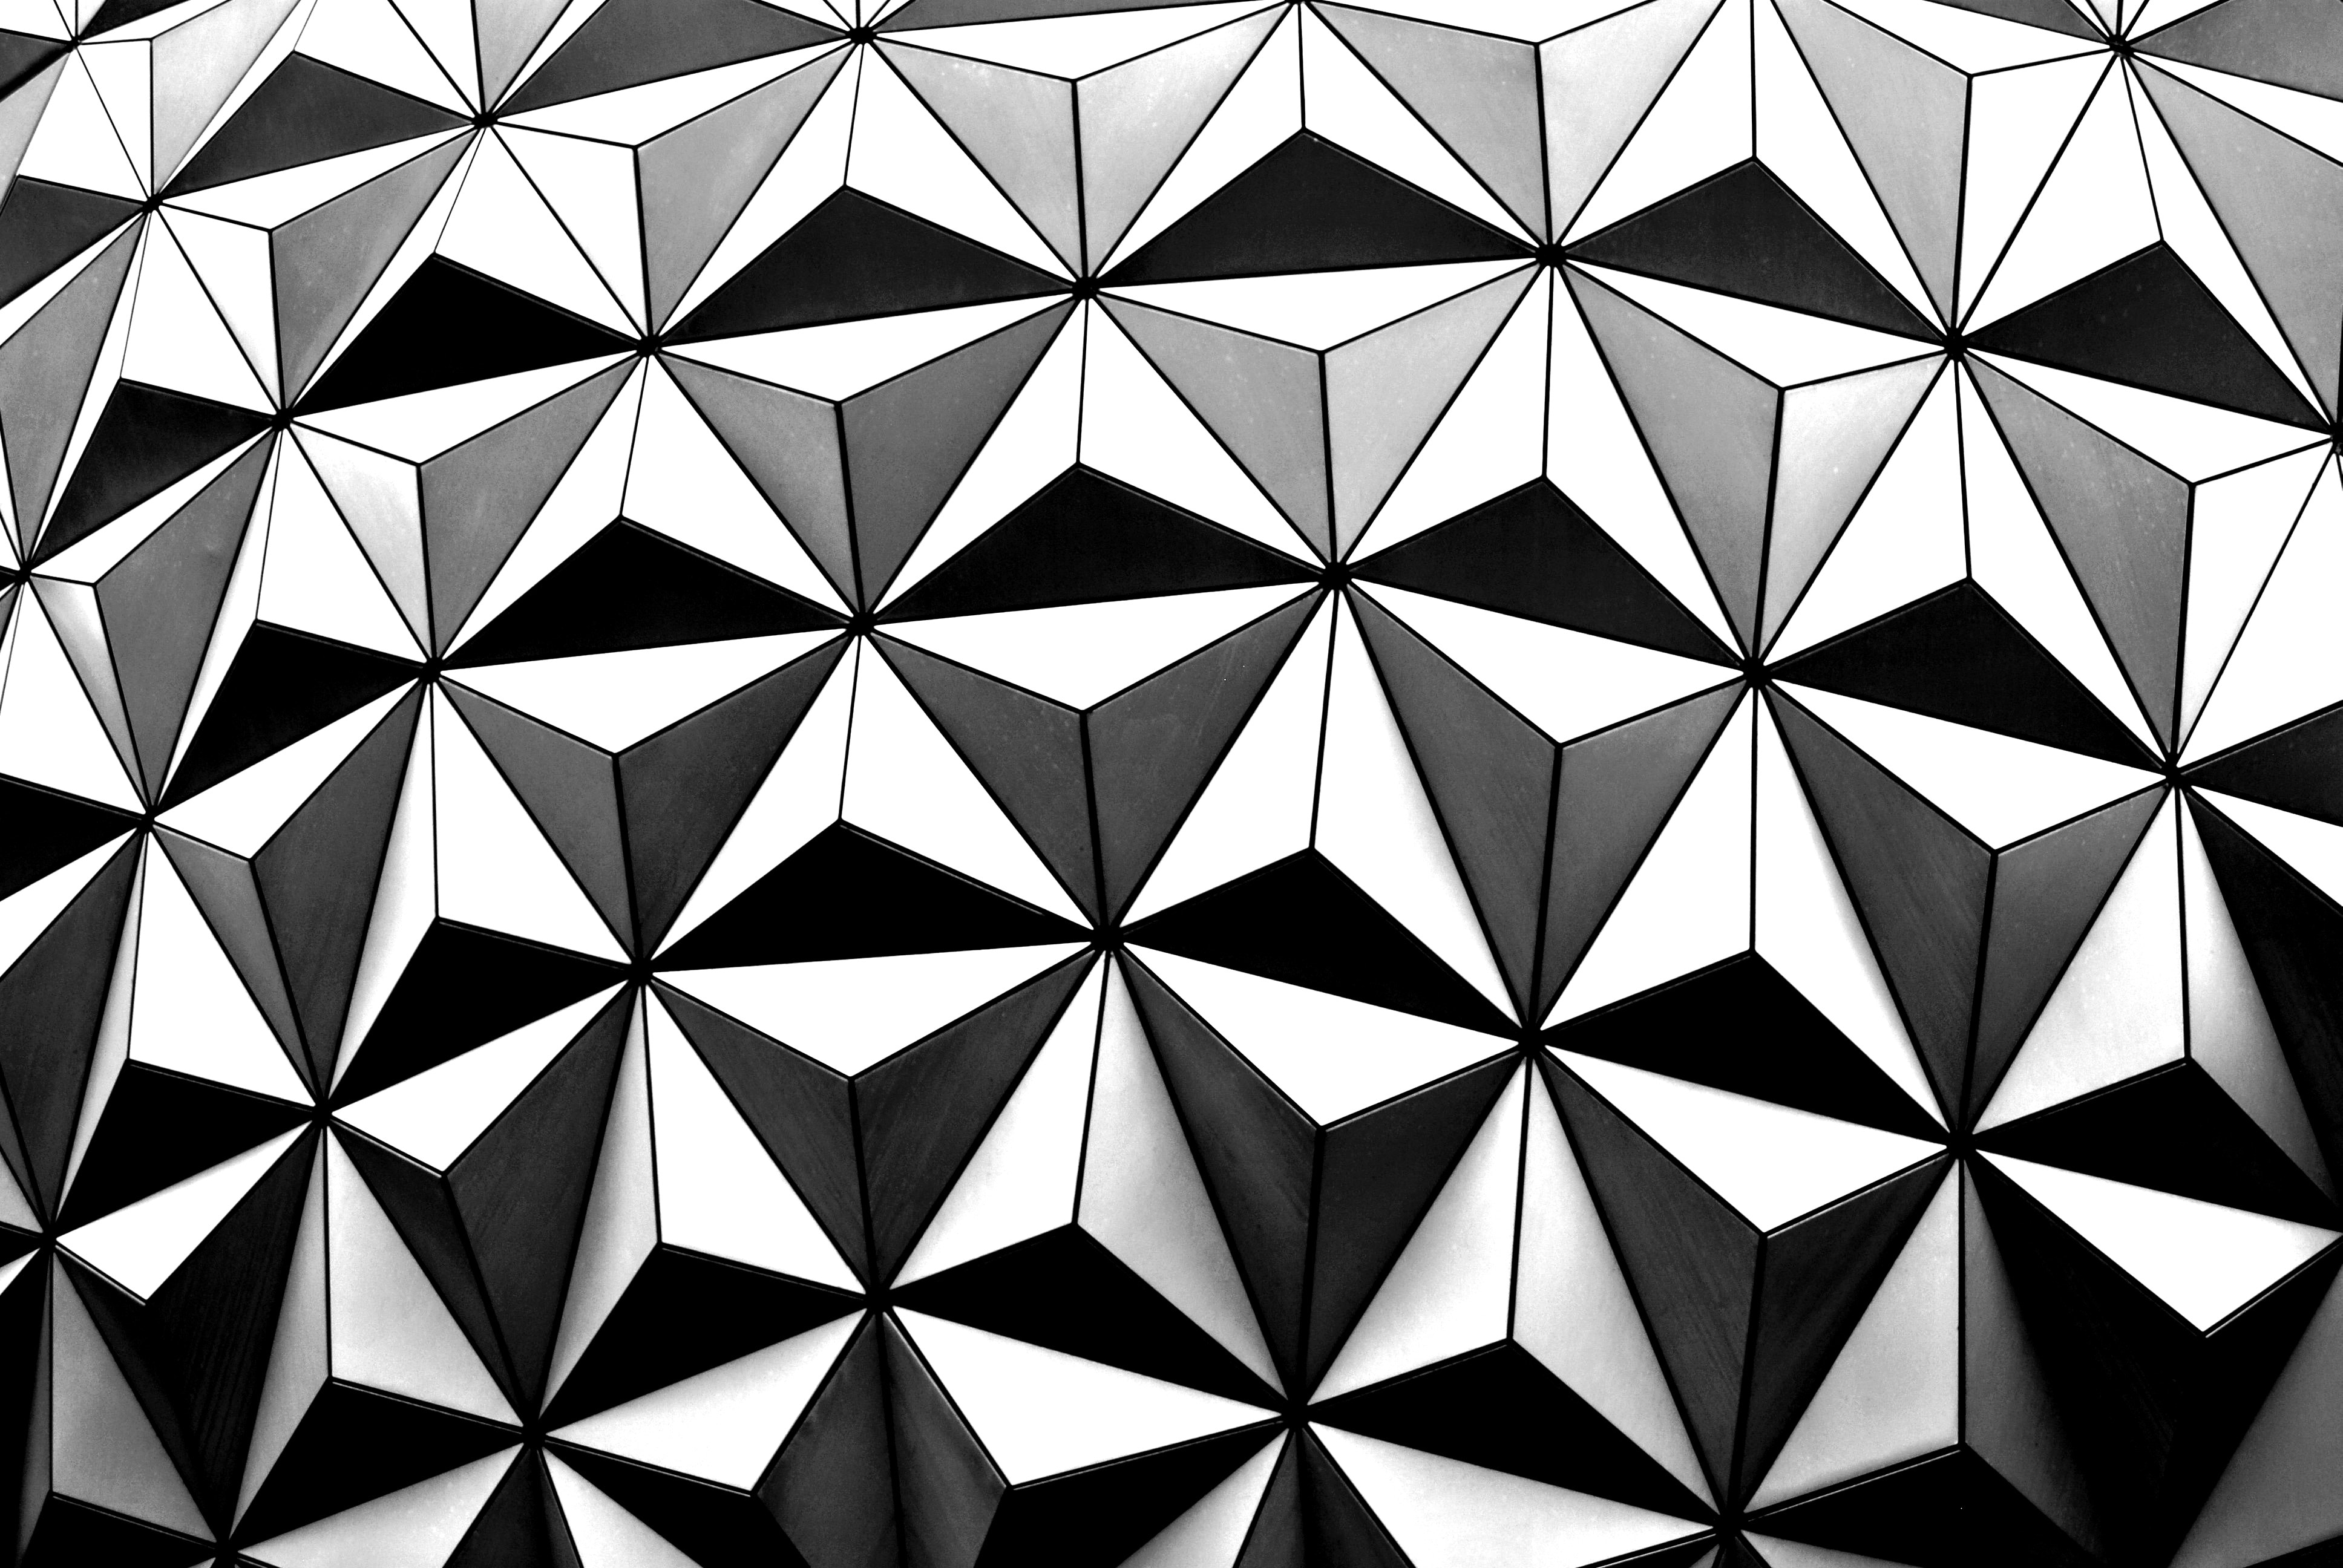
\includegraphics[height = 6\baselineskip]{./assets/abstract-abstract-photo-art-1070345.jpg}
					\caption{}
					\label{subfig:06-01-sponge}
				\end{subfigure}%
				\begin{subfigure}{0.5\columnwidth}
					\centering
					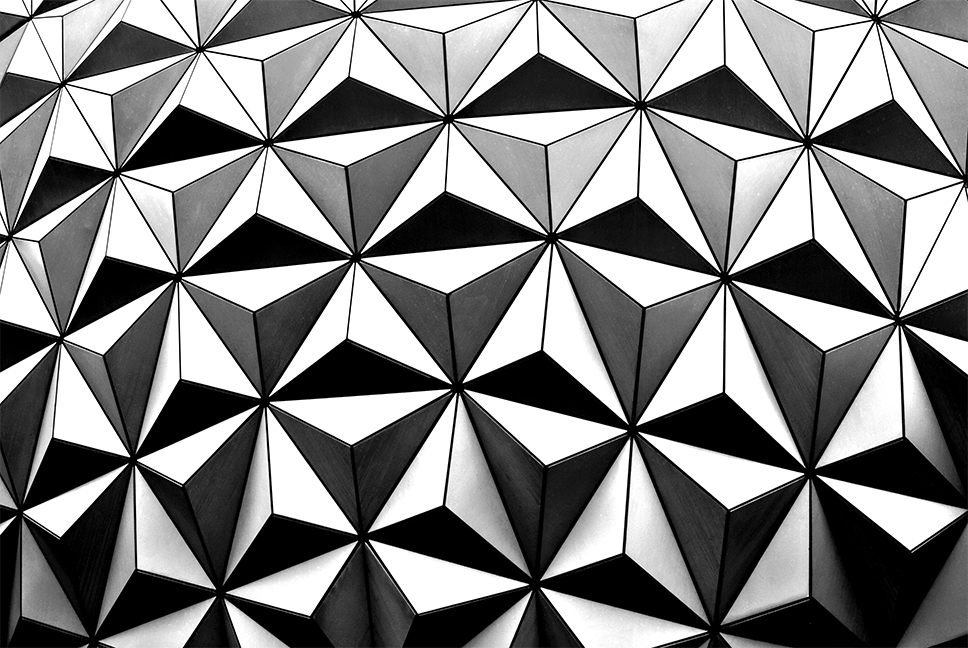
\includegraphics[height = 6\baselineskip]{./assets/y03s01-multimedia-lab-01-p01-06-sponge.jpg}
					\caption{}
					\label{subfig:06-02-sponge}
				\end{subfigure}%
				\caption{Результат роботи команди~\textenglish{«Sponge»}: \subref{subfig:06-01-sponge}~— до, \subref{subfig:06-02-sponge}~— після}
				\label{fig:06-sponge}
			\end{figure}

		\paragraph{Освітлювач}
			Створюємо шар під~назвою~\textenglish{«Dodge\&Burn»} та~виконуємо над~ним операції~\textenglish{«Dodge»} та~\textenglish{«Burn»}~(рис.~\ref{fig:07-dodge-burn}).
			\begin{figure}[!htbp]
				\centering
				\begin{subfigure}{0.5\columnwidth}
					\centering
					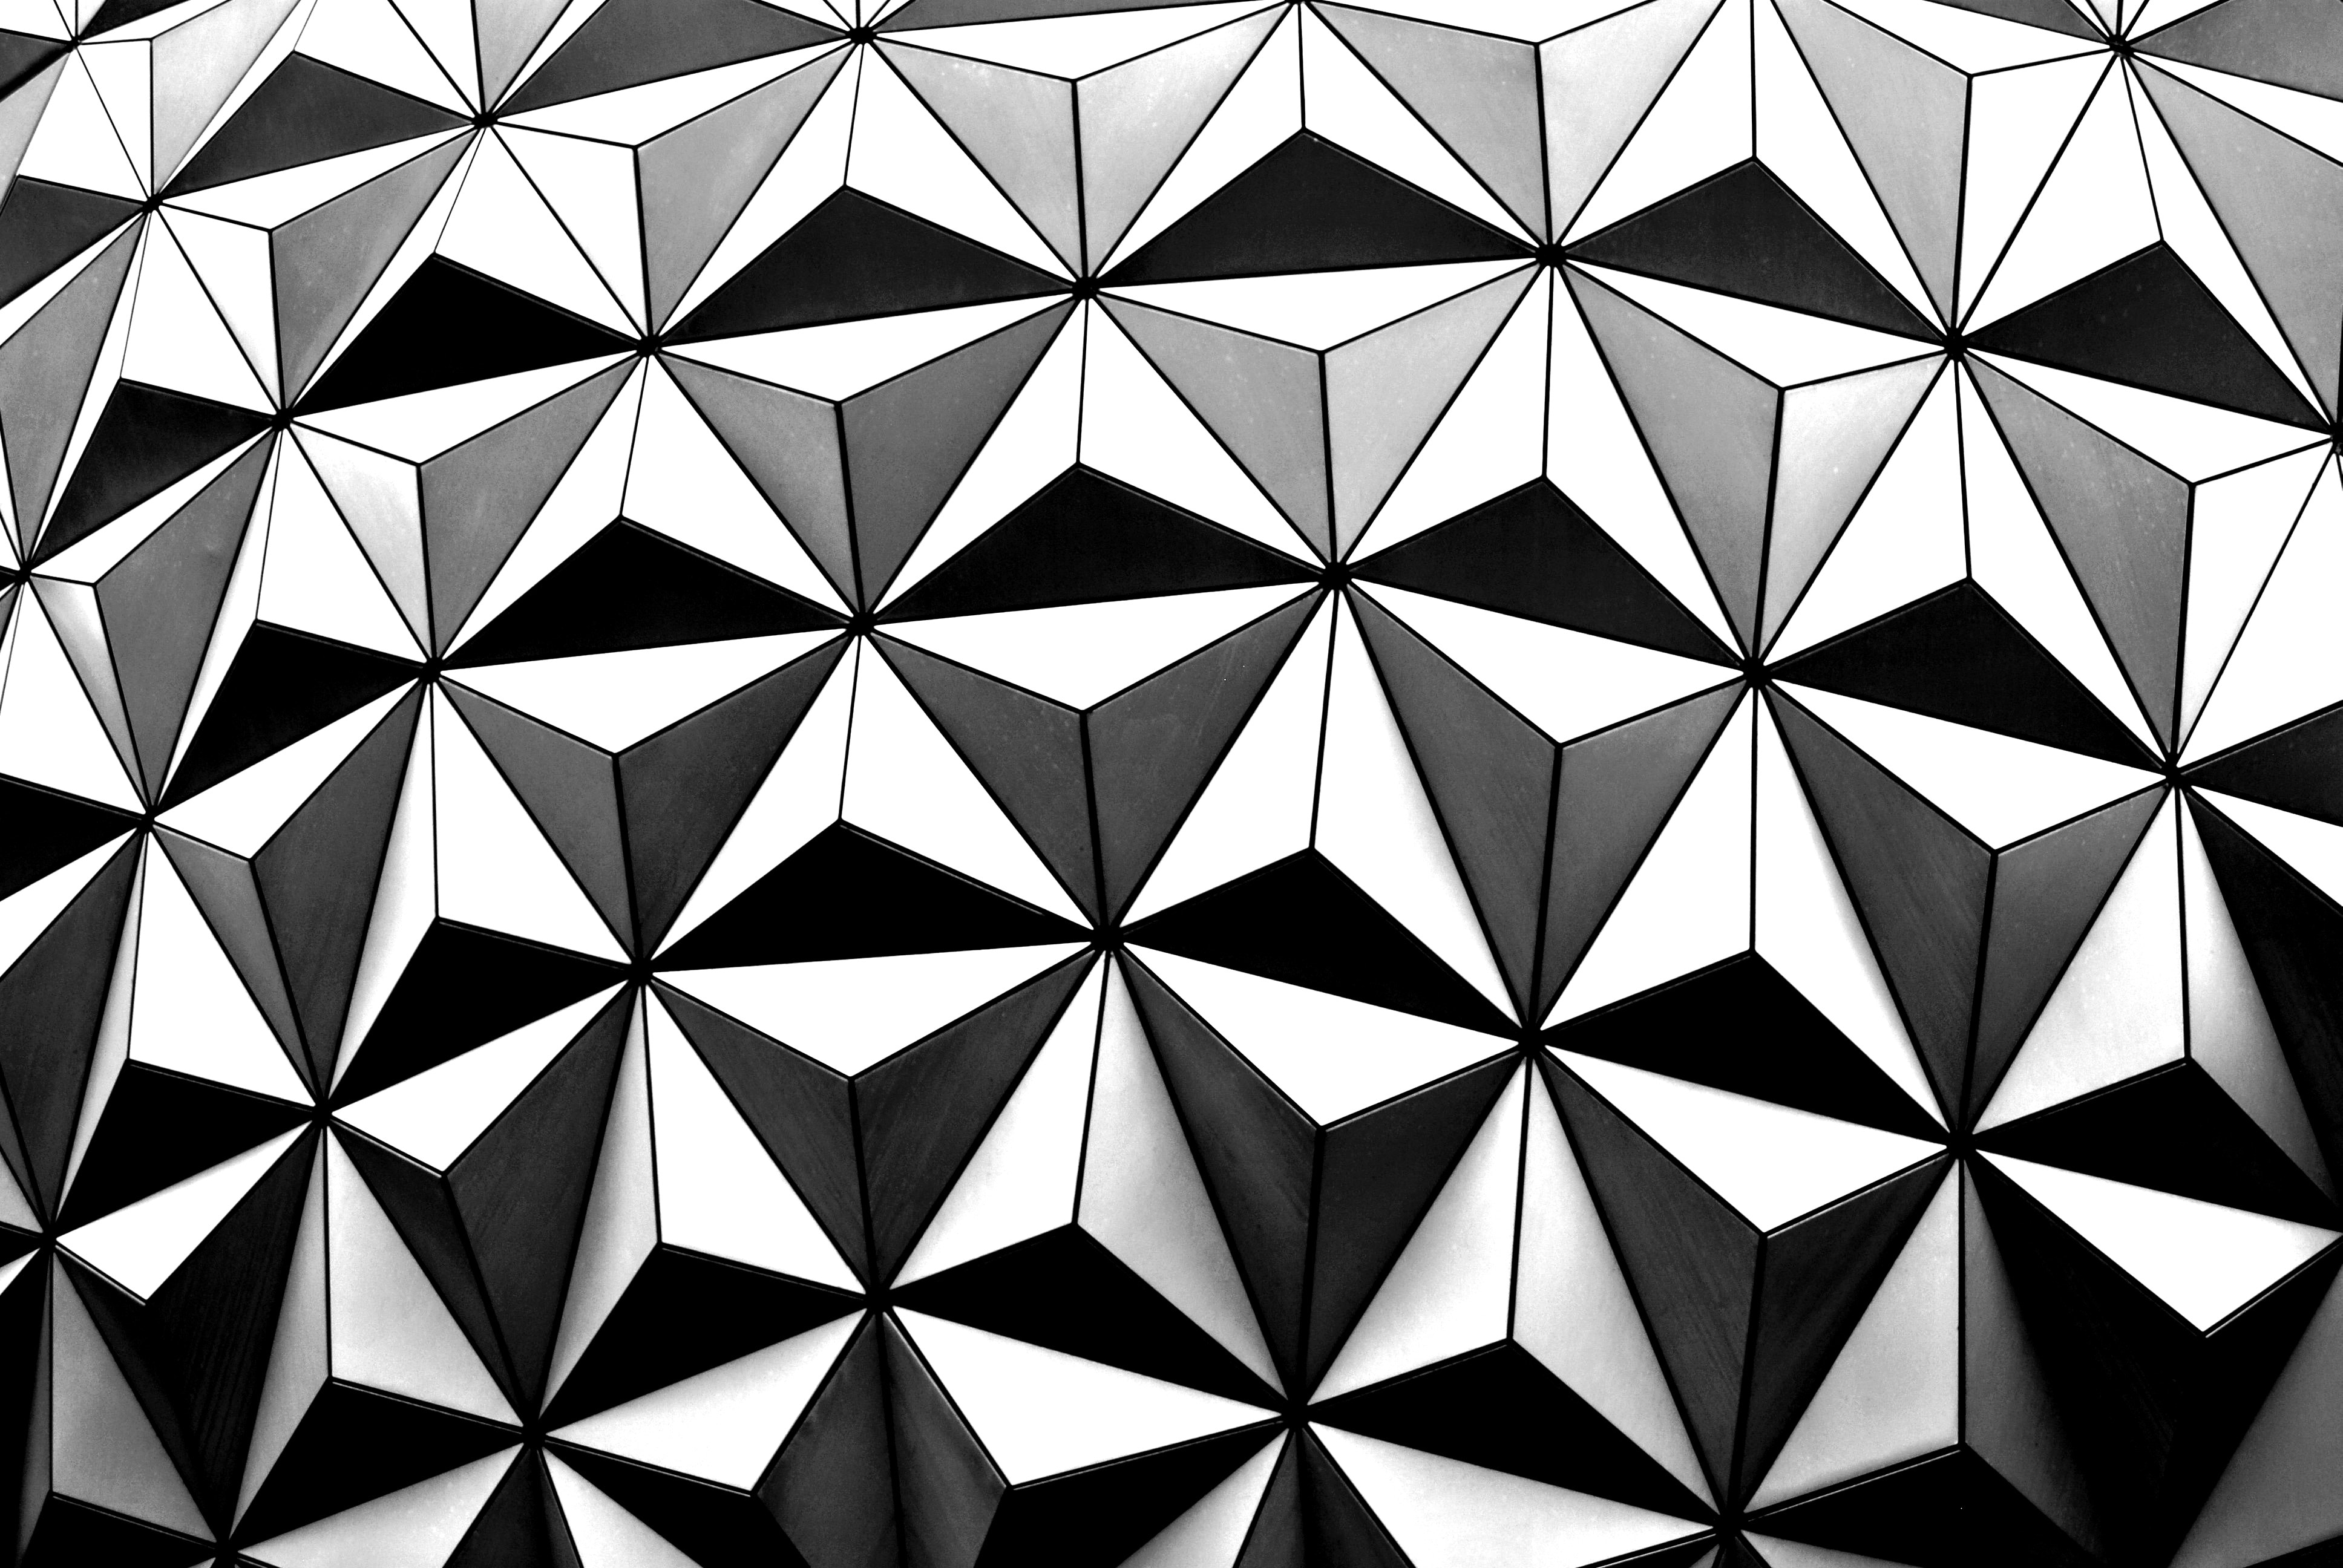
\includegraphics[height = 6\baselineskip]{./assets/abstract-abstract-photo-art-1070345.jpg}
					\caption{}
					\label{subfig:07-01-dodge-burn}
				\end{subfigure}%
				\begin{subfigure}{0.5\columnwidth}
					\centering
					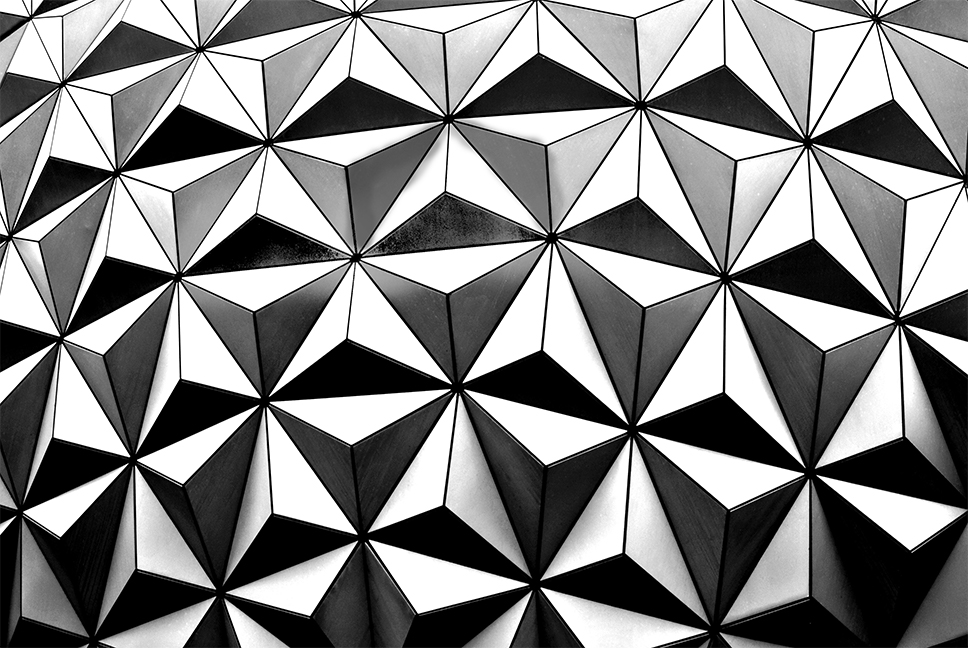
\includegraphics[height = 6\baselineskip]{./assets/y03s01-multimedia-lab-01-p01-07-dodge-burn.jpg}
					\caption{}
					\label{subfig:07-02-dodge-burn}
				\end{subfigure}%
				\caption{Результат роботи команд~\textenglish{«Dodge»} та~\textenglish{«Burn»}: \subref{subfig:07-01-dodge-burn}~— до, \subref{subfig:07-02-dodge-burn}~— після}
				\label{fig:07-dodge-burn}
			\end{figure}

	\section{Висновок}
		Виконуючи дану лабораторну роботу ми~вивчили інтерфейс програми~\textenglish{Adobe Photoshop} і~ознайомились з~основними інструментами для~редагування зображень.

\end{document}
